% Generated by code/needham.py -- do not edit by hand.
\definecolor{qocA}{rgb}{0.00,0.45,0.70}
\definecolor{qocB}{rgb}{0.90,0.60,0.00}
\definecolor{qocC}{rgb}{0.00,0.62,0.45}
\definecolor{qocD}{rgb}{0.80,0.40,0.00}
\definecolor{qocE}{rgb}{0.80,0.60,0.70}
\definecolor{qocF}{rgb}{0.35,0.70,0.90}
\begin{tikzpicture}[ink/.style={line width=0.9pt, ndInk}, faint/.style={line width=0.4pt, ndInk!35}, dashedink/.style={line width=0.5pt, ndInk!55, dash pattern=on 2.5pt off 2pt}, vec/.style={->, >=stealth, line width=1.2pt}, note/.style={font=\footnotesize\itshape, text=ndInk!85, align=center}, pointer/.style={->, >=stealth, line width=0.4pt, ndInk!60, shorten >=2pt, shorten <=1pt}, dot/.style={circle, fill=ndInk, inner sep=0pt, minimum size=3.4pt}, wash/.style={fill=ndSky, fill opacity=0.55}, every node/.style={text=ndInk}]
\definecolor{ndInk}{rgb}{0.13,0.13,0.18}
\definecolor{ndPaper}{rgb}{0.99,0.96,0.88}
\definecolor{ndSky}{rgb}{0.84,0.91,0.98}
\definecolor{ndRose}{rgb}{0.98,0.86,0.84}
\definecolor{ndBlue}{rgb}{0.13,0.36,0.66}
\definecolor{ndRed}{rgb}{0.78,0.20,0.16}
\definecolor{ndGold}{rgb}{0.88,0.62,0.10}
\definecolor{ndGreen}{rgb}{0.18,0.52,0.30}
\fill[ndRose, fill opacity=0.85] (-2.076,1.311) -- (-1.348,-1.110) -- (1.348,-2.254) -- cycle;
\fill[ndSky, fill opacity=0.95] (-1.712,0.100) -- (0.000,-1.682) -- (-0.364,-0.472) -- cycle;
\fill[ndRose, fill opacity=0.85] (2.076,2.054) -- (-2.076,1.311) -- (1.348,-2.254) -- cycle;
\fill[ndSky, fill opacity=0.95] (0.000,1.682) -- (-0.364,-0.472) -- (1.712,-0.100) -- cycle;
\draw[line width=0.5pt, ndBlue!70, densely dashed] (0.364,0.472) -- (-1.712,0.100);
\draw[line width=0.5pt, ndBlue!70, densely dashed] (0.364,0.472) -- (1.712,-0.100);
\draw[line width=0.5pt, ndBlue!70, densely dashed] (0.364,0.472) -- (0.000,1.682);
\draw[line width=0.5pt, ndBlue!70, densely dashed] (0.364,0.472) -- (0.000,-1.682);
\draw[line width=0.8pt, ndBlue] (-0.364,-0.472) -- (-1.712,0.100);
\draw[line width=0.8pt, ndBlue] (-0.364,-0.472) -- (1.712,-0.100);
\draw[line width=0.8pt, ndBlue] (-0.364,-0.472) -- (0.000,1.682);
\draw[line width=0.8pt, ndBlue] (-0.364,-0.472) -- (0.000,-1.682);
\draw[line width=0.5pt, ndBlue!70, densely dashed] (-1.712,0.100) -- (0.000,1.682);
\draw[line width=0.8pt, ndBlue] (-1.712,0.100) -- (0.000,-1.682);
\draw[line width=0.8pt, ndBlue] (1.712,-0.100) -- (0.000,1.682);
\draw[line width=0.5pt, ndBlue!70, densely dashed] (1.712,-0.100) -- (0.000,-1.682);
\draw[ink] (2.076,2.054) -- (-2.076,1.311);
\draw[dashedink] (2.076,2.054) -- (-1.348,-1.110);
\draw[ink] (2.076,2.054) -- (1.348,-2.254);
\draw[ink] (-2.076,1.311) -- (-1.348,-1.110);
\draw[ink] (-2.076,1.311) -- (1.348,-2.254);
\draw[ink] (-1.348,-1.110) -- (1.348,-2.254);
\draw[faint, ->, >=stealth, ndInk!60] (-3.100,-2.100) -- (-2.944,-1.898) node[anchor=west, font=\scriptsize, text=ndInk] {$\langle XX\rangle$};
\draw[faint, ->, >=stealth, ndInk!60] (-3.100,-2.100) -- (-3.834,-2.057) node[anchor=east, font=\scriptsize, text=ndInk] {$\langle YY\rangle$};
\draw[faint, ->, >=stealth, ndInk!60] (-3.100,-2.100) -- (-3.100,-1.379) node[anchor=south, font=\scriptsize, text=ndInk] {$\langle ZZ\rangle$};
\draw[ndRed, line width=1.0pt, densely dashed] (0.000,0.000) -- (0.449,-0.751);
\draw[ndRed, line width=1.2pt] (0.449,-0.751) -- (1.348,-2.254);
\node[dot, fill=ndRed, minimum size=4pt] at (0.449,-0.751) {};
\node[dot, minimum size=3pt] at (0.000,0.000) {};
\node[font=\small, anchor=east, fill=ndSky, inner sep=1pt] at (-0.060,0.000) {$\tfrac14\Id$};
\node[dot, fill=ndRed, minimum size=3.6pt] at (2.076,2.054) {};
\node[font=\small] at (2.303,2.279) {$\Phi^{+}$};
\node[dot, fill=ndRed, minimum size=3.6pt] at (-2.076,1.311) {};
\node[font=\small] at (-2.346,1.482) {$\Phi^{-}$};
\node[dot, fill=ndRed, minimum size=3.6pt] at (-1.348,-1.110) {};
\node[font=\small] at (-1.595,-1.314) {$\Psi^{+}$};
\node[dot, fill=ndRed, minimum size=3.6pt] at (1.348,-2.254) {};
\node[font=\small] at (1.512,-2.529) {$\Psi^{-}$};
\node[dot, fill=ndBlue, minimum size=3.4pt] at (0.000,1.682) {};
\node[note, anchor=south east] (cc) at (-0.350,2.282) {$\tfrac12(\ket{00}\bra{00}+\ket{11}\bra{11})$:\\ classically correlated};
\draw[pointer] (cc.south east) to[bend left=12] (-0.040,1.732);
\node[note, anchor=north west, text=ndRed] (w) at (1.449,-1.901) {Werner states $t=-p(1,1,1)$:\\ separable for $p\le\frac13$};
\draw[pointer] (w.north west) to[bend left=12] (0.499,-0.801);
\node[note, anchor=east, text=ndBlue] (s) at (-1.798,-0.010) {separable:\\ $\abs{t_1}+\abs{t_2}+\abs{t_3}\le1$,\\ the octahedron};
\draw[pointer] (s.east) to[bend left=12] (-0.692,-0.685);
\node[note, anchor=west, text=ndRed!80!ndInk] (en) at (2.276,0.954) {entangled:\\ the four corners};
\draw[pointer] (en.west) to[bend left=12] (1.588,1.549);
\end{tikzpicture}
